Shotwell jest domyślnym menadżerem zdjęć w systemie Ubuntu. Jego zadaniem jest dbanie o organizacje twojej kolekcji fotografi i plików graficznych. Przy pierwszym uruchomieniu Shotwell zaproponuje zaimportowanie wszystkich zdjęć z katalogu Obrazy znajdującym się w twoim katalogu domowym. W przyszłości fotografie wrzucane do tego katalogu będa automatycznie dodawane do kolekcji w programie Shotwell.
\begin{center}
	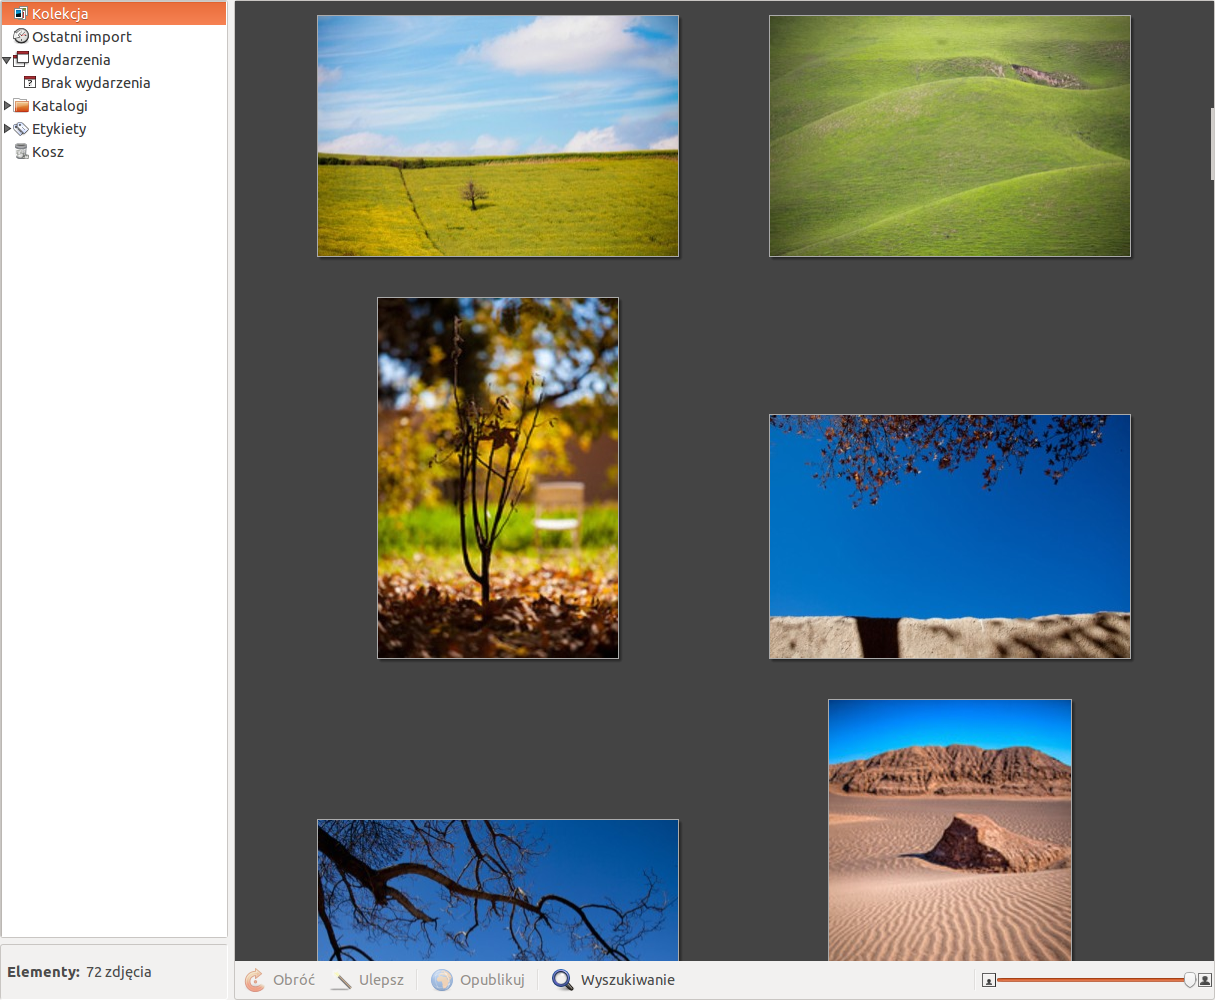
\includegraphics[width=\linewidth]{images/programy_shotwell1.png}
\end{center}

Główne okno programu shotwell składa się z trzech częśći:
\begin{itemize}
\item \textcolor{ubuntu_orange}{Lewy panel} zawierający skróty do zaimportowanych katalogów i głównej kolekcji.
\item \textcolor{ubuntu_orange}{Główny obszar} ze wszystkimi brazkami w aktualnie wybranej kolekcji.
\item \textcolor{ubuntu_orange}{Pasek narzedziowy} zawierający narzedzia umożliwiające korekcję zdjęć.
\end{itemize}
\subsubsection{Podstawy obsługi programu Shotwell}
Dodawanie zdjęć do kolekcji
\begin{itemize}
\item Umieść zdjęcia w katalogu Obrazu automatycznie dodać je do kolekcji programu Shotwell.
\item Wejdź w \menu{{Plik}>{Zaimportuj z katalogu\ldots}} aby wskazać nowy katalog. Będziesz mieć wybór pomiędzy zwykłym importem ze wskazanego katalogu (zdjęcia zostaną dopisane do twojej kolekcji i pozostaną w oryginalnym katalogu) lub skopiowaniem ich do katalogu Obrazy.
\item Wejdź w \menu{{Plik}>{Zaimportuj z programu\ldots}} aby zaimportować bazę zdjęć z innego programu zainstalowanego na twoim komputerze.
\end{itemize}
Zaznaczanie zdjęć:
\begin{itemize}
\item Kliknij lewym przyciskiem myszy na zdjęcie aby je zaznaczyć.
\item Kliknij dwa razy lewym przyciskiem myszy aby przejść do widoku pojedyńczego zdjęcia.
\item Wciśnij \keys{Shift} i kliknij lewym przyciskiem myszy aby zaznaczyć wiele kolejnych zdjęć.
\item Wciśnij \keys{CTRL} i klikaj lewym przyciskiem myszy aby zaznaczyć konkretne zdjęcia.
\item Kliknij prawym przyciskiem myszy aby wyświetlić menu kontekstowe zdjęcia.
\end{itemize}
Eksport zdjęć:
\begin{itemize}
\item Zaznacz zdjęcia, które chesz wyeksportować
\item Wejdź w \menu{{Plik}>{Wyeksportuj}} aby wskazać katalog do którego zdjęcia mają być skopiowane.
\item Wejdź w \menu{{Plik}>{Opublikuj}} aby opublikować zdjęcia w serwisie internetowym. Obsługę dodatkowych serwisów możesz dodać w programie \textcolor{ubuntu_orange}{Konta sieciowe}.
\item Wejdź w \menu{{Plik}>{Wyślij do\ldots}} aby móc wyeksportować zdjęcia do
	\begin{itemize}
	\item \textcolor{ubuntu_orange}{Dyski wymienne i zasoby sieciowe} - pozwala wybrać miejsce docelowe dla zdjęć w sieci lokalnej lub na lokalnie podłączonych urzadzeniach (np. dysk USB)
	\item \textcolor{ubuntu_orange}{Asystent CD?DVD} - uruchamia program do wypalania pły Brasero i umożliwia nagranie wybranych zdjęć na płytę optyczną.
	\item \textcolor{ubuntu_orange}{Wiadomość} - umożliwia wysłanie zdjęć poprzez komunikator internetowy (np. Empathy).
	\item \textcolor{ubuntu_orange}{BlueToth} - wysyła zdjecia bezprzewodowo do urzadzeń Bluetooth.
	\item \textcolor{ubuntu_orange}{E-mail} - otwiera program pocztowy i dodaje zdjęcia jako załączniki.
	\end{itemize}	
\end{itemize}
